% ====================================== %
% Chapter: Bezpečné použití kryptografie %
% Status: Final                          %
% ====================================== %
\label{pouziti}

Přestože jsou dnes používané kryptografické algoritmy bezpečné v~teorii, nemusí to nutně znamenat, že jsou vždy bezpečné i~v~praxi. Kryptografie je obzvláště náročná na správnou implementaci a~kryptografický kód je obecně složitější než kód ne-kryptografický. Bezpečná implementace kryptografie vyžaduje od programátora specifické znalosti a~je proto obzvláště náchylná na vznik zranitelností, které mohou mít v~tomto případě naprosto devastující následky. Střední doba mezi vznikem a~opravou zranitelnosti v~kryptografických implementacích se navíc pohybuje v~řádu jednotek let, což dává útočníkům poměrně široké časové okno na jejich nalezení a~zneužití.~\cite{youreallyshouldnt}

Ani bezpečné implementace kryptografických algoritmů bez jakýchkoli zranitelností ale nejsou postačující podmínkou pro bezpečné použití kryptografie v~softwaru. Naopak se ukazuje, že nejprominentnějším bezpečnostním problémem souvisejícím s~kryptografií nejsou zranitelné implementace kryptografických algoritmů, ale situace, kdy vývojář použije správně implementovaný kryptografický algoritmus špatným způsobem~\cite{das2014iv} --- takové případy měly mezi lety~2011--2014 na svědomí až 83~\% kryptografických zranitelností v~databázích CVE~\cite{lazaretal}. Komplexní rozhraní kryptografických knihoven jsou často pro vývojáře nesrozumitelná~\cite{hurdles} a~to vede k~vysokému počtu případů zranitelného použití kryptografie v~softwaru~\cite{comparative2023}. V~roce~2019 například bylo zjištěno, že přes 72~\% open-source projektů v~jazyce Java alespoň jedním způsobem chybně pracuje s~kryptografií~\cite{javacrypto}. K~podobně znepokojivým závěrům dochází studie zranitelností v~aplikacích pro systém Android~\cite{egele-android} a~mnoho dalších (stručný přehled poskytují Luo a~kol.~\cite{comparative2023}). Nabízí se tedy otázka, jestli mohou kryptografické knihovny (například kvalitou své dokumentace, návrhem rozhraní, atd.) chybnému použití ze strany svých uživatelů předcházet.

\begin{figure}[!ht]
    \centering
    \label{img-devs-crypto}
    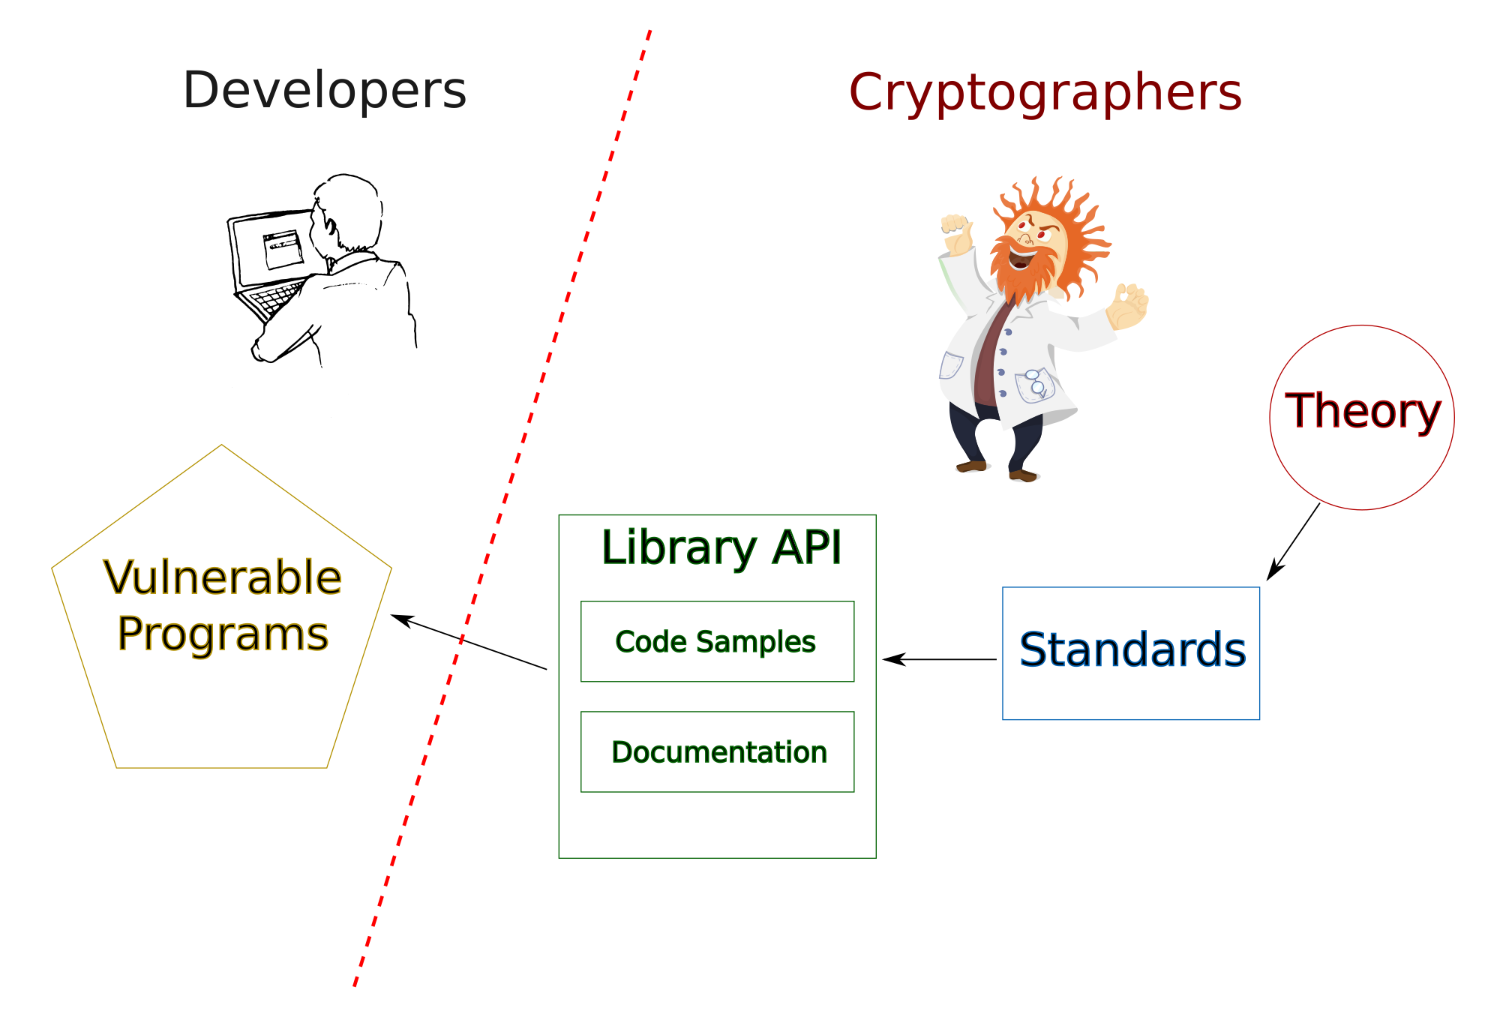
\includegraphics[width=0.8\textwidth]{text/media/developers_cryptographers.png}
    \caption[~Začlenění kryptografie do softwarového vývoje]{Začlenění kryptografie do softwarového vývoje podceňuje rozdíl mezi expertízou kryptografů a~vývojářů. Převzato z~\cite{das2014iv}.}
\end{figure}

\section{Kryptografická primitiva a kryptografické protokoly}

Než shrneme zjištění získaná literární rešerší problematiky bezpečného (resp.\ zranitelného) po\-u\-ži\-tí kryptografie v~kódu, při\-po\-me\-ne\-me pro čtenářovo pohodlí některé základní kryptografické algoritmy běžně používané v~dnešních aplikacích a~některé jejich důležité charakteristiky relevantní pro jejich bezpečné použití. Tyto kryptografické algoritmy lze zjednodušeně rozdělit na dvě kategorie: První kategorií jsou kryptografická primitiva, tedy jakési stavební kameny kryptografie, druhou jsou kryptografické protokoly, tj.~úplné specifikace zabezpečené komunikace.

\subsubsection*{Symetrická šifra a její autentizace}

Symetrická šifra je kryptografické primitivum sloužící k~utajení informace. Toho dosahuje šif\-ro\-va\-cí transformací, která pomocí tajného klíče převádí otevřený text (OT) na šifrový text (ŠT), a~k~ní inverzní de\-šif\-ro\-va\-cí transformací. Ta pro úspěšné dešifrování zprávy vyžaduje v~případě symetrické šifry použití téhož klíče, kterým byla zpráva zašifrována.

Základní vlastností, kterou od dnešních symetrických šifer očekáváme, je IND-CPA neboli \emph{nerozlišitelnost při útoku s~výběrem otevřeného textu} (angl.~\textit{indistinguishability under chosen-plaintext attack}):

\begin{definition}[IND-CPA]
    Vlastnost IND-CPA symetrické šifry je definována jako neschopnost pomyslného nepřítele uspět v~následující hře:

    Nepřítel libovolně zvolí dva OT, které jsou následně zašifrovány (stejným) neznámým klíčem. Dále má nepřítel k~dispozici šifrovací orákulum\footnote{Orákulum je v~informatice obecně termín pro stroj s~neznámou implementací, který se ale chová deterministicky, tj.~na daný vstup vždy odpoví stejným výstupem. Šifrovací orákulum tedy umožňuje nepříteli zašifrovat libovolný otevřený text bez prozrazení tajného klíče.} (ale ne samotný klíč). Pokud nepřítel ani v~takové situaci prokazatelně nedokáže s~významnou pravděpodobností rozeznat, který ŠT přísluší kterému OT, pak o~šifře řekneme, že je IND-CPA.~\cite{das2014iv}
\end{definition}

Dnes používané konstrukce symetrických šifer, které jsou schopné za určitých podmínek tuto vlastnost zaručit, rozdělujeme na šifry \emph{proudové} a~\emph{blokové}.

Proudové šifry z~klíče pevné velikosti deterministicky generují \emph{posloupnost hesla} (v~angličtině \textit{keystream}), která určuje transformace jednotlivých znaků při šifrování a~dešifrování zprávy. Aby šifra splnila vlastnost IND-CPA, je ale potřeba zajistit, že při opakovaném použití stejného šifrovacího klíče nedojde k~vygenerování totožné posloupnosti hesla a~tedy totožných substitucí. Za tímto účelem do vlastního šifrovacího a~dešifrovacího algoritmu vstupuje zpravidla kromě klíče a~OT/ŠT ještě \emph{inicializační vektor} (IV) --- nepředvídatelná jednorázová hodnota (\textit{number used once} neboli zkráceně \textit{nonce}), která zaručuje jedinečnost posloupností hesel napříč šifrováními. Inicializační vektor je veřejný parametr --- pro pozdější úspěšné dešifrování zprávy musí být adresátovi předán spolu s~šifrovým textem.

Blokové šifry na rozdíl od těch proudových negenerují nekonečnou posloupnost hesla; kryptoanalýze brání tak, že zprávu šifrují po blocích většího počtu znaků najednou (dnes nejčastěji 128 bitů, tj.\ 16 bajtů). Vzhledem k~tomu, že (de)šifrovací transformace bloku závisí pouze na klíči, pro dosažení IND-CPA nestačí zprávu jednoduše rozdělit na bloky příslušné velikosti a~každý blok zašifrovat zvlášť. Uvažme například blokovou šifru nad českou abecedou s~mezerou a~interpunkcí, velikost bloku 4~znaky a~otevřený text \texttt{ZDAR, NAZDAR}. Šifrování by proběhlo zvlášť nad bloky ``\texttt{ZDAR}'', ``\texttt{, NA}'' a~``\texttt{ZDAR}'' --- to znamená, že první a~poslední blok šifrového textu by byly shodné. Z~toho by útočník dokázal usoudit, že šifrovaná zpráva nemůže být žádná taková, kde první blok není shodný s~posledním, což by mu výrazně zlehčilo prolomení šifry.\footnote{Didakticky tento problém demonstruje fenomén ``ECB tučňáka'' popsaný například v~\cite{ecbpenguin}.}

Řešením tohoto problému (a~mnoha dalších, které by takové použití přinášelo) a~tedy dů\-le\-ži\-tým prostředkem pro bezpečné použití blokových šifer jsou \emph{operační módy} (někdy též \emph{provozní režimy}, angl.\ \textit{modes of operation}). Triviální operační mód, který každý blok OT zašifruje zvlášť toutéž transformací (a~tedy nesplňuje IND-CPA), se nazývá \textit{electronic codebook mode}, zkr.~ECB. Za bezpečné\footnote{Za určitých podmínek.} jsou považovány z~klasických operačních módů například \textit{cipher block chaining mode} (CBC), \textit{cipher feedback mode} (CFB) a~\textit{output feedback mode} (OFB), které z~podobného důvodu jako proudové šifry navíc vyžadují jako vstup inicializační vektor. Vedle klasických operačních módů navíc existují i~operační módy se zvláštním účelem, např.\ \textit{XEX-based tweaked-codebook mode with ciphertext stealing} (XTS) speciálně navržený pro šifrování disků nebo tzv.~autentizované módy \textit{Galois/counter mode} (GCM), \textit{counter with CBC-MAC} (CCM) a~mód EAX, jejichž význam popíšeme vzápětí.

Samotné šifrování ne\-do\-ká\-že komunikaci zcela zabezpečit: Zaprvé nezaručuje integritu a~autenticitu tajných zpráv, zadruhé je jeho použití možné pouze v~případě, že se již dříve obě strany domluvily na tajném klíči. První z~těchto problémů byl v~aplikované kryptografii tradičně řešen explicitním použitím MAC funkcí (\textit{message authentication code}), které na základě dat a~tajného klíče vypočtou kód pevné velikosti, který slouží jako důkaz pravosti a~nepoškozenosti zprávy. Určité vylepšení nad tímto postupem přinášejí \emph{autentizované šifry}, které kombinují použití symetrické šifry a~MAC do jednoho algoritmu, resp.\ do jedné abstrakce. Výstupem šifrování je kromě šifrového textu \emph{autentizační tag}, který musí být spolu s~ŠT předán dešifrovacímu algoritmu. Pokud útočník šifrový text za přenosu modifikuje, tag vypočtený při dešifrování se nebude shodovat s~tím přijatým a~dešifrování selže. Některé autentizované šifry navíc nabízejí autentizaci tzv.~\emph{asociovaných dat}, tedy části zprávy, která není šifrována.~\cite{Dworkin2007}

Mezi rozšířené symetrické šifry, které jsou dnes považovány za bezpečné, patří proudové šifry ChaCha20 a~Salsa20, bloková šifra AES (\textit{Advanced Encryption Standard}) a~na nich založená AEAD schémata\footnote{\textit{Authenticated Encryption with Associated Data}.} ChaCha20-Poly1305 a~AES v~jednom z~autentizovaných módů zmíněných výše (nejčastěji GCM). Z~již prolomených, ale historicky hojně používaných symetrických šifer stojí za zmínku především proudová šifra RC4 (Arcfour) a~bloková šifra DES (\textit{Data Encryption Standard}).

\subsubsection*{Asymetrická kryptografie}

V~předchozích odstavcích jsme popsali šifrovací systémy, které pro šifrování i~dešifrování používají shodný klíč. Takové schéma umožňuje utajit komunikaci dvou ``rovnocenných'' stran, ale nepokryje situace, kdy požadujeme například, aby jeden účastník komunikace mohl zprávu zašifrovat (podepsat) a~kdokoli jiný ji mohl posléze dešifrovat (podpis ověřit), aniž by ale mohl sám takový šifrový text (podpis) vytvořit. Další problém, který nám asymetrická kryptografie pomáhá vyřešit, je problém ustanovení klíče: Aby strany mohly vůbec utajit komunikaci po ne\-za\-bez\-pe\-če\-ném kanále, musí se nejdřív dohodnout na tajném a~ne\-před\-ví\-da\-tel\-ném společném klíči.

Jedním z~nejstarších, přesto dodnes používaným algoritmem pro asymetrické šifrování a~podepisování je RSA (Rivest-Shamir-Adleman) založený na modulárním mocnění v~konečném tělese. Jeho bezpečnost stojí na složitosti problému faktorizace modulu --- součinu dvou velmi velkých prvočísel, které zná pouze vlastník soukromého klíče. Dalším rozšířeným algoritmem pro digitální podepisování je \emph{Digital Signature Algorithm} (DSA) založený na (klasickém) problému diskrétního logaritmu\footnote{Tj.~nalezení logaritmu zadaného čísla při zadaném základu v~konečném tělese.} a~jeho modernější verze (ECDSA, EdDSA) využívající eliptické křivky.

Pro ustanovení společného klíče pro symetrické šifrování přes nezabezpečený kanál se používá zpravidla některá varianta algoritmu \emph{Diffie-Hellman}. Podobně jako u~DSA existují dvě varianty: Starší z~nich je založená na klasickém problému diskrétního logaritmu, v~současnosti preferovaná je varianta s~eliptickými křivkami (\textit{Elliptic Curve Diffie-Hellman}, ECDH)~\cite{haakegaard2015elliptic}.

\subsubsection*{Hašovací funkce a funkce pro odvození klíče}

Kryptografické hašovací funkce jsou jednosměrné bezkolizní funkce, které libovolně velkým datům přiřadí číslo pevné velikosti (případně velikosti, která je zadána jako vstupní parametr\footnote{Např.\ algoritmus BLAKE3 podporuje výstup libovolné velikosti.}). Jejich jednosměrnost spočívá v~tom, že ze znalosti obrazu (výstupu\footnote{Výstup kryptografické hašovací funkce se označuje jako \emph{hash}, případně \emph{fingerprint}, \emph{message digest} (MD) nebo \emph{manipulation detection code} (MDC).}) nelze efektivně (v~polynomiálním čase) vypočíst vzor (vstup); bezkoliznost znamená, že neexistuje efektivní algoritmus pro nalezení libovolných dvou vzorů se stejným obrazem (odolnost proti kolizi 1.~druhu) a~speciálně k~pevně zadanému vzoru nelze efektivně nalézt jiný vzor se stejným obrazem (kolize 2.~druhu). Hašovací funkce slouží jako důkazy o~integritě zpráv a~lze pomocí nich např.\ konstruovat MAC funkce (tzv.~\textit{hash-based} MAC neboli HMAC). Za určitých předpokladů mohou hašovací funkce sloužit také k~ověření znalosti nějaké informace bez toho, aby tato informace byla explicitně uchovávána (např.\ uživatelské heslo v~databázi).

Funkce pro odvození klíče (\textit{Key Derivation Function}, KDF) jsou podobné hašovacím funkcím v~tom smyslu, že na základě libovolně dlouhého vstupu (hesla) vyprodukují nepředvídatelný řetězec zadané délky. Jejich návrh ale zároveň zpravidla zahrnuje záměrně výpočetně náročnou operaci (např.\ iterovanou aplikaci hašovací funkce) za účelem zamezení útokům hrubou silou (\textit{brute-force attack}) a~náhodnou sůl (\textit{salt}) jako obranu proti slovníkovým útokům (\textit{dictionary attack} nebo přesněji \textit{rainbow table attack}).

Mezi dnes běžně používané kryptografické hašovací funkce patří především různé varianty algoritmu \emph{Secure Hashing Algoritm} (SHA) --- s~výjimkou SHA-1, pro který byla v~roce 2017 nalezena kolize 1.~druhu~\cite{shattered} --- a~dále např.\ algoritmy BLAKE, RIPEMD, bcrypt nebo Argon. Pro odvození klíče z~hesla se dnes standardně používá funkce PBKDF2 (\textit{Password-Based Key Derivation Function 2}), která kromě hesla a~soli jako vstupní parametry přijímá počet iterací, hešovací funkci a~požadovanou délku výstupu~\cite{rfc2898}. 

\subsubsection*{Generátory náhodných čísel}

Generování náhodných, resp.\ pseudonáhodných čísel (RNG, resp.\ PRNG) není samo o~sobě kryptografickou operací, bez\-peč\-nost mnoha kryptografických algoritmů se však právě od kvality zdroje náhodnosti odvíjí. Například od klíče pro symetrickou šifru očekáváme maximální entropii, jinými slovy chceme, aby útočníkovi pro prolomení šifry (i~se znalostí použitého generátoru) nezbylo nic lepšího, než vyzkoušet všechny binární řetězce příslušné délky. Konkrétně od \emph{kryptograficky bezpečných generátorů pseudonáhodných čísel} (CSPRNG) vyžadujeme dvě základní vlastnosti --- nepředvídatelnost dalšího bitu na základě jakékoli známé posloupnosti předchozích bitů (\textit{next-bit test}) a~nemožnost rekonstrukce předchozí hodnoty pseudonáhodné posloupnosti na základě zjištění vnitřního stavu (\textit{state compromise}).~\cite{csprng}

Výchozí pseudonáhodné generátory ve standardních knihovnách programovacích jazyků ale takovou kvalitu zpravidla neposkytují, neboť jejich účelem není bezpečnost, ale rychlost --- ve většině situací mimo kryptografii postačuje pouze \emph{zdánlivě nepředvídatelná} náhodnost.

\subsubsection*{Protokol TLS}

\textit{Transport Layer Security} (TLS) je kryptografický protokol, který ``\textit{umožňuje aplikacím s~architekturou klient–server komunikovat přes internet způsobem, který zabraňuje odposlechu, manipulaci a~falšování zpráv}''~\cite{tls13rfc}. K~tomu TLS využívá mimo jiné kryptografická primitiva popsaná výše.

Použití TLS obnáší především dvě specifika. Prvním z~nich je volba správné verze protokolu --- verze TLS 1.1 a~starší\footnote{Včetně protokolu SSL (\textit{Secure Sockets Layer}), který je předchůdcem TLS.} jsou ze své podstaty zranitelné vůči různým druhům útoků, které v~nejhorším případě dokážou šifrování (resp.\ autentizaci a~integritu) úplně prolomit~\cite{poodle}. V~dnešních aplikacích je proto nutné používat výhradně TLS verze 1.2 nebo 1.3.

Druhým specifikem použití protokolu TLS je autentizace serveru vůči klientovi, případně výjimečně i~klienta vůči serveru. Zahájení komunikace mezi klientem a~serverem probíhá v~TLS protokolu prostřednictvím \textit{TLS handshake}, v~jehož průběhu mimo jiné server pošle klientovi svůj certifikát, neboli doklad o~pravosti jeho veřejného klíče podepsaný \emph{certifikační autoritou}. Klient posléze musí tento certifikát validovat, aby se ujistil, že není falešný nebo neplatný. Zaprvé musí na základě sady kořenových certifikátů ověřit řetěz certifikace a~ověřit pravost certifikátu, dále musí validovat datum expirace certifikátu a~ověřit, že certifikát nebyl certifikační autoritou revokován. Validace certifikátu je stručně řečeno složitým --- a~jak uvidíme později, pro vývojáře aplikací problematickým~\cite{comparing2017} --- úkolem, přičemž její nesprávná implementace může v~nejhorším případě útočníkovi poskytnout příležitost pro velmi přímočarý útok typu \textit{man-in-the-middle}.

\section{Návrh kryptografických rozhraní}

Prvním významným aspektem bezpečnosti kryptografických knihoven je návrh jejího pro\-g\-ra\-má\-tor\-ského rozhraní. Autoři Green a~Smith v~článku~\cite{greensmith} z~roku 2016 poukazují na závažnost chyb, kterých se vývojáři dopouštějí při práci s~kryptografií, a~formulují 10 doporučení pro bezpečný návrh kryptografických rozhraní. Poznamenávají, že kryptografická rozhraní pro programování aplikací (\emph{Application Programming Interface}, API) jsou specifická především tím, že jejich špatné použití nevede k~tak viditelným chybám jako chybné použití ne-kryptografických API, a~proto je jejich zneužití mnohem hůře identifikovatelné. Zároveň připomínají, že vytváření snadno použitelných bezpečnostních mechanismů je lepším prostředkem pro zabránění vzniku chyb, než vzdělávání uživatelů, aby dokázali bezpečně pracovat se softwarem, který je složitý a~matoucí. Mezi svých 10 doporučení pro návrh kryptografických API zařazují především:

\begin{itemize}
    \item \textbf{Kryptografie má být zahrnuta do standardních API.} \enskip
        Autoři vychází ze skutečnosti, že vývojáři typicky nepřemýšlí v~kryptografických termínech --- svůj problém neformulují jako výměnu klíčů pomocí asymetrického kryptografického schématu, validaci certifikátu a~volbu blokové symetrické šifry, jejího operačního modu a~autentizačního mechanismu. Vývojáři chtějí typicky řešit problémy jako je navázání tajné komunikace s~dalším zařízením, stáhnutí a~ověření integrity souboru z~vzdáleného serveru, bezpečné uložení hesla do databáze, zašifrování souboru pomocí hesla, apod. Pokud je kryptografický protokol enkapsulovaný ve standardním API, např.\ API pro komunikaci pomocí HTTPS nebo SSH, pak je problém s~chybným použitím kryptografie koncovým vývojářem téměř zcela eliminován.

    \item \textbf{API musí být dostatečně flexibilní.} \enskip
        V~situaci, kdy API neumožňuje dostatečně flexibilní použití, aby pomocí něj vývojář dosáhl svého cíle, se může stát (a~podle zkušeností autorů se tak skutečně děje), že se bude vývojář pokoušet daný bezpečnostní mechanismus obcházet nebo ho nějakým způsobem ohýbat, což přirozeně zvyšuje riziko vzniku chyby.

    \item \textbf{API musí být srozumitelné i~pro ne-experty.} \enskip
        Kryptografie je složitá, ale její složitost lze v~mnoha případech před jejími uživateli skrýt. Pokud knihovna po uživateli například vyžaduje explicitně specifikovat operační mód, který má být použitý při šifrování algoritmem AES, zvyšuje se tím šance, že vývojář použije nebezpečný mód, např.\ ECB~\cite{comparing2017}. Podobně pokud bude knihovna po uživateli vyžadovat při šifrování hodnotu inicializačního vektoru, snadno se stane, že vývojář použije pokaždé stejnou konstantní nebo snadno predikovatelnou hodnotu a~tím nevědomě kompromituje kvalitu šifrování~\cite{das2014iv}.

        Autoři proto doporučují kryptografické detaily schovat do implementace a~uživateli z\-pří\-stup\-nit vysokoúrovňové API, které nebude vyžadovat detailní znalost kryptografie.

    \item \textbf{API musí být obtížné použít špatně.} \enskip
        Podle autorů by návrháři kryptografických API měli vyvinout co největší úsilí pro to, aby nesprávnému použití API úplně předcházeli; implementace by se zase měly za běhu snažit nesprávné použití detekovat a~případně vyvolat chybu/výjimku. Zdůrazňují, že chyby by měly být zřetelné, srozumitelné, a~nemělo by být možné je snadno obejít či vypnout (nebo by alespoň mechanismus umožňující chybu obejít měl být explicitně označen jako nebezpečný).

    \item \textbf{Výchozí parametry musí být bezpečné a~jednoznačné.} \enskip
        Většina uživatelů softwaru použije jeho výchozí konfiguraci~\cite{Daswani2007}, je tedy vysoce žádoucí, aby taková konfigurace nepoužívala slabé parametry, nebo v~nejhorším případě parametry, které naprosto anulují bez\-peč\-nost\-ní záruky daného kryptografického algoritmu.

        Jako odstrašující příklad lze použít knihovnu PyCrypto. Před tím, než byl v~roce 2013 její vývoj ukončen, dlouho plnila roli de facto standardní kryptografické knihovny pro jazyk Python~\cite{keckmasters}, byť z~hlediska kvality API trpěla vážnými nedostatky. Například její funkce pro vytvoření objektu pro šifrování algoritmem AES měla nepovinný parametr \texttt{IV} reprezentující inicializační vektor, o~kterém dokumentace knihovny píše, že pokud jej programátor nespecifikuje, tak se použije výchozí hodnota se samými nulami~\cite{pycryptodoc}. Stejně nebezpečný byl výchozí operační mód pro šifrování blokovými šiframi, kterým byl mód ECB~\cite{das2014iv}.

        S~podobným problém se potýkalo i~kryptografické rozhraní Java Cryptography Architecture (JCA), které po uživateli sice nevyžadovalo explicitně nastavit operační mód šifry, ale výchozí hodnota byla ponechána na implementaci, přičemž některé implementace jako výchozí hodnotu zvolily opět zranitelný mód ECB~\cite{greensmith}.

    \item \textbf{Knihovna by měla nabízet testovací mód.} \enskip
        Další doporučení vychází z~poznatku, že vývojáři často chtějí svůj kód testovat deterministicky a~bez dopadu na výkon a~složitost kódu, který mohou bezpečnostní mechanismy do programu vnést. To je může vést k~tomu, že pro účely testování bezpečnostní mechanismy úplně vypnou nebo použijí parametry, které kvalitní knihovna vyhodnotí jako zranitelné (např.\ statický IV nebo klíč). Takové požadavky podle autorů nejsou nesmyslné, protože náhodnost obecně ztěžuje testování kódu. U~konvenčních řešení však hrozí scénář, že vývojáři například zapomenou po testování bezpečnost opět posílit a~nedopatřením vydají software používající takto oslabenou testovací konfiguraci. Autoři proto navrhují do knihoven zavést zvláštní testovací mód, který bude možné např.\ svázat s~konkrétním identifikátorem stroje, na kterém se kód bude testovat.

        Autoři nicméně uvádí, že v~době publikace si nejsou vědomi žádné knihovny, která by takovou funkcionalitu nabízela.
\end{itemize}

Návrhem kryptografických API se zabývají i~další autoři. Konkrétně studie~\cite{comparing2017, comparative2023} se zabývají porovnáním knihoven, které se snaží použití kryptografie zjednodušit, s~tradičními kryptografickými knihovnami. Důležitým závěrem jejich výzkumu je pozorování, že samotná jednoduchost API použití knihovny nezjednodušuje, pokud knihovně chybí kvalitní dokumentace nebo nepokrývá dostatečně široké spektrum použití~\cite{comparing2017}.

Zajímavým pokusem o~pokrok v~bezpečnosti a~použitelnosti kryptografických API (při zachování jejich flexibility) představuje knihovna FluentCrypto popsaná v~článku~\cite{fluentcrypto} z~roku~2021. Samotná knihovna měla poskytovat alternativní rozhraní ke kryptografickému modulu runtimu Node.js, zajímavou ji ale činí především její přístup k~volbě kryptografických algoritmů a~jejich parametrů. Do procesu výběru kryptografických parametrů měli vstupovat tři aktéři: Prvním aktérem byli experti na kryptografii, kteří pomocí zvláštní syntaxe v~tzv.\ ``CryRule'' souborech popsali pravidla, resp.\ omezení, kterými se použití kryptografie muselo řídit (např.\ povolené šifry, operační módy, délky klíčů, atd.). Druhým aktérem byli aplikační vývojáři, kteří pouze použili rozhraní knihovny způsobem, který jim dával smysl. (Rozhraní knihovny bylo zároveň navrženo tak, aby bylo jeho intuitivní použití s~implicitními parametry bezpečné, ale přesto umožňovalo pokročilou konfiguraci.) Posledním aktérem byl samotný runtime knihovny, který za doby běhu kontroloval soulad volání API s~definovanými požadavky. Přestože v~experimentech porovnávajících FluentCrypto s~výchozím rozhraním pro kryptografii v~Node.js knihovna dosahovala pozoruhodných výsledků~\cite{fluentcrypto}, z~důvodů, které nám nejsou známé, bohužel projekt FluentCrypto již není aktivní (odkaz na repositář knihovny v~článku je nefunkční a~její kód nelze ani jinak dohledat). Přesto se nám jeho přístup k~návrhu kryptografických knihoven a~jejich rozhraní zdá být velmi slibný.

\section{Programovací jazyky}

Problematikou chyb v~použití kryptografie se dále zabývají autoři Das a~kol., kteří v~článku~\cite{das2014iv} z~roku~2014 z\-kou\-ma\-jí kryptografické knihovny ze 7~úhlů (opakované použití IV, výchozí hodnoty, zahlcení funkcemi, chybějící funkce, dokumentace, ukázkový kód a~programovací jazyk) a~formulují doporučení pro budoucí vývoj kryptografických knihoven. Na jejich výzkum navazují Luo a~kol.\ článkem~\cite{comparative2023} z~roku~2023, v~němž skrze řízený experiment porovnávají použitelnost rozhraní pro symetrickou kryptografii 9~růz\-ných kryptografických knihoven a~opět formulují doporučení pro bezpečně použitelné kryptografické knihovny. Obě zmíněné studie se mimo jiné dotýkají volby programovacího jazyka, ve kterém knihovna svoje rozhraní nabízí, a~zdůrazňují výhody \emph{paměťově bezpečných} a~\emph{silně typovaných} jazyků, resp.\ rozhraní.

\subsection{Paměťová bezpečnost}

Každý program potřebuje ke svému běhu určité množství paměti, do které si ukládá např.\ vstup od uživatele, mezivýsledky výpočtů pro pozdější zpracování, stav vykonávání programu, apod. Různé programovací jazyky přitom poskytují různé úrovně abstrakce nad prací se ``surovou'' pamětí prostřednictvím proměnných, struktur, polí, objektů, atd. Relevantní jsou pro nás tři aspekty paměťové bezpečnosti: dynamická alokace paměti, která může vést ke zranitelnostem typu \textit{use-after-free}, dále kontrola přístupu do paměti (\textit{bounds checking}), bez které je snadné do programu vnést zranitelnosti typu \textit{přetečení bufferu}, a~nakonec neinicializovaná paměť, která může především způsobit \textit{vyzrazení důvěrných informací}.

Nízkoúrovňové jazyky, konkrétně jazyky symbolických instrukcí (angl.\ \textit{assembly languages}) a~jazyk C (potažmo C++), poskytují pouze velmi základní abstrakce nad pamětí v~podobě proměnných a~jejich typů. Starost o~správnou (a~bezpečnou) práci s~pamětí je v~těchto jazycích zodpovědností jejich uživatele. Dynamické alokace a~dealokace paměti programátor v~těchto jazycích dosáhne explicitním voláním API standardní knihovny (případně operačního systému); správná inicializace proměnných a~kontrola toho, že program nepřistupuje na adresy mimo rozsah paměti alokované pro data programu, je také ponechána na programátorovi. Jazyk C (a~do určité míry C++) je díky svojí jednoduchosti bezkonkurenčně výkonný a~dodnes široce používaný mj.\ v~implementacích operačních systémů, v~softwaru pro vestavěné systémy, apod., jeho nevýhodou ale je, že explicitní práce s~pamětí je náchylná na chyby a~z~hlediska bezpečnosti tudíž velmi riziková~\cite{gaynor2020} --- dokonce se ukazuje, že v~kryptografických knihovnách napsaných v~jazyce C a~C++ převažují zranitelnosti způsobené chybnou prací s~pamětí nad chybami kteréhokoli jiného druhu a~konstituují přes 37~\% zranitelností v~těchto knihovnách~\cite{youreallyshouldnt}.

Jazyky, které bývají označovány jako vysokoúrovňové, složitost (dynamické) alokace paměti před uživatelem schovávají jedním z~mnoha možných způsobů. Programy v~jazycích, které jsou interpretované (např.\ Python, JavaScript nebo PHP), se z~principu nemusí alokací paměti vůbec zabývat, protože ji obsluhuje běhové prostředí jejich interpretu. Dalším způsobem, jak abstrahovat (de)alokaci paměti, je mechanismus zvaný \textit{garbage collection} (GC), který dealokaci již nepotřebných bloků paměti ponechává na běhovém prostředí, které si uchovává seznam alokovaných bloků paměti a~platných odkazů na ně. (Mezi jazyky využívající tento přístup patří třeba jazyky Java nebo Go.) Poslední paměťovou abstrakcí hodnou zmínky je koncept vlastnictví paměti (\textit{ownership}) a~mechanismus \textit{borrow checking}, jehož průkopníkem je programovací jazyk Rust. V~tomto modelu má každá alokovaná proměnná svou ``vlastnící'' funkci a~jazyk za doby překladu vynucuje sadu pravidel pro její ``vypůjčování''. Takový přístup kombinuje bezpečnost vysokoúrovňových jazyků s~výkonem nízkoúrovňových jazyků, jeho záruky ale nejsou stoprocentní\footnote{V~některých krajních případech překladač \texttt{rustc} nechá uživatele napsat kód, který s~pamětí pracuje špatně~\cite{cvers}.}.

Paměťově bezpečné jazyky jako Python, Java nebo (do určité míry) Rust zároveň uživateli nedovolí přistoupit k~nealokované paměti (např.\ před začátek nebo za konec pole), například tím, že při takovém pokusu vyvolají výjimku (Python, Java), paniku (Rust) nebo vrátí zvláštní hodnotu (\texttt{undefined} v~JavaScriptu). Podobnými mechanismy takové jazyky zabrání programu číst neinicializovanou paměť. Takovými opatřeními tyto jazyky zabraňují tomu, aby vývojář vlastní vinou do své aplikace vnesl paměťovou chybu (přetečení bufferu, use-after-free, apod.). Do aplikací se takové chyby mohou stále dostat skrze zranitelnosti v~běhovém prostředí jazyka, implementaci překladače nebo knihovně samotného jazyka, takové situace jsou ale podstatně vzácnější --- už jen proto, že programovacích jazyků je výrazně méně než jejich uživatelů.

\subsection{Slabé a silné typování}

Dalším aspektem programovacích jazyků, který může potenciálně mít vliv na bezpečné použití (nejen) kryptografických knihoven, je jeho typový systém, neboli způsob, kterým programovací jazyk zaručuje správnost datových typů proměnných.

\begin{lstlisting}[caption={[~Rozhraní funkce pro inicializaci šifry v~knihovně OpenSSL]~Rozhraní funkce pro inicializaci šifry v~knihovně OpenSSL \cite{openssl-evp-encryptinit}},label={lst:openssl-evp-encryptinit},float,language=C]
int EVP_EncryptInit_ex(EVP_CIPHER_CTX *ctx,
                       const EVP_CIPHER *type,
                       ENGINE *impl,
                       const unsigned char *key,
                       const unsigned char *iv);
\end{lstlisting}

\begin{lstlisting}[caption={[~Rozhraní funkce pro inicializaci šifry v~Java Cryptography Architecture]~Rozhraní funkce pro inicializaci šifry v~Java Cryptography Architecture \cite{jca-encryptinit}},label={lst:jca-encryptinit},float,language=Java]
public void init(int opmode, Key key, AlgorithmParameters params);
\end{lstlisting}

Luo a~kol.~\cite{comparative2023} tuto problematiku demonstrují na příkladu rozhraní pro inicializaci symetrických šifer. Výpis kódu~\ref{lst:openssl-evp-encryptinit} ukazuje hlavičku funkce pro inicializaci symetrické šifry v~knihovně OpenSSL, výpis~\ref{lst:jca-encryptinit} deklaraci analogické funkce v~specifikaci Java Cryptography Architecture. Zatímco v~JCA knihovna explicitně rozlišuje typy šifrovacího klíče a~parametrů odvíjejících se od použitého algoritmu (tj.~je \emph{silně typuje}), funkce knihovny OpenSSL z~hlediska typů vůbec nerozlišuje mezi klíčem a~inicializačním vektorem. ``Slabé'' typování parametrů zvyšuje riziko, že je uživatel nedopatřením obmění nebo alokuje nesprávné množství paměti; pokud je typem ukazatel na \texttt{unsigned char} (namísto dedikovaného typu reprezentující pole bajtů), může to v~některých uživatelích navíc vyvolat dojem, že vstupem má být textový řetězec~\cite{comparative2023}.

Tendence vývojářů používat silné typy je přirozenou výhodou objektově-orientovaného programování (OOP) typického pro jazyk Java, objektový návrh ale není nutnou podmínkou pro použití silných typů. Výpis kódu \ref{lst:c-strong-types} představuje jeden možný způsob, kterým by šly (s~nulovou penalizací z~hlediska výkonu programu) odlišit typy pro klíč a~IV i~v~jazyce C.

\begin{lstlisting}[caption={~Možná implementace silných typů pro klíč a~IV v~jazyce C},label={lst:c-strong-types},float,language=C]
#include <stdint.h>
#include <stdlib.h>

constexpr size_t KEY_LENGTH = /* ... */;
struct Key { const uint8_t bytes[KEY_LENGTH]; };

constexpr size_t IV_LENGTH = /* ... */;
struct IV { const uint8_t bytes[IV_LENGTH]; };
\end{lstlisting}

Takové ``silné typy'' nabízejí vedle rozlišení jednotlivých parametrů funkcí a~zaručení správ\-ných velikostí polí ale i~další výhody.  Například v~jazycích podporujících zapouzdření (tedy rozlišení ``soukromých'' a~``veřejných'' členů struktur) lze takto vynutit, aby klíče nebo nonce byly konstruovány specifickým způsobem. Zatímco struktury z~výpisu~\ref{lst:c-strong-types} v~jazyce C uživatel může instancovat přímo (výpis~\ref{lst:c-instantiation}), například v~jazyce Rust lze využít implicitně soukromých členů struktur a~uživatele tak donutit IV vytvořit jednou z~funkcí, které nabízí její implementace (výpisy~\ref{lst:rust-encapsulation} a~\ref{lst:rust-instantiation}).

\begin{lstlisting}[caption={~Přímá inicializace struktury IV v~jazyce C},label={lst:c-instantiation},float,language=C]
int main(void)
{
    struct IV iv = {{0}};
    
    // ...
}
\end{lstlisting}

\begin{lstlisting}[caption={~Možné zapouzdření IV v~jazyce Rust},label={lst:rust-encapsulation},float]
mod cipher {
    pub const IV_LENGTH: usize = /* ... */;

    pub struct IV { bytes: [u8; IV_LENGTH] }

    impl IV {
        pub fn new_random() -> Self
        {
            // ...
        }
    }
}
\end{lstlisting}

\begin{lstlisting}[caption={~Nemožnost přímé inicializace zapouzdřeného IV v~jazyce Rust},label={lst:rust-instantiation},float]
fn main()
{
    /* This will not compile - 'bytes' is a private field. */
    let iv = cipher::IV { bytes: [0_u8; cipher::IV_LENGTH] };

    /* OK */
    let iv = cipher::IV::new_random();

    // ...
}
\end{lstlisting}

Opomenout nesmíme ani \emph{dynamicky typované} jazyky, tedy jazyky, které informaci o~typu proměnných zpracovávají nikoli staticky za doby překladu, ale dynamicky za doby běhu. Takové jazyky (z~těch populárních např.\ Python nebo JavaScript) umožňují typy proměnných měnit v~průběhu vykonávání programu a~nelze je proto snadno staticky validovat. U~takových jazyků nemá dobrý smysl hovořit o~silném nebo slabém typování; v~případě kryptografických knihoven těchto jazyků je zkrátka zodpovědností implementace, aby správnost argumentů funkce zkontrolovala v~době její invokace.

\section{Zdroje informací}

Dalším aspektem použití kryptografických knihoven, který se ukazuje být kritickým pro jejich (ne)bez\-peč\-nost, jsou zdroje informací, ze kterých může jejich uživatel vyjít. Plasticky toto demonstrují experimentální výzkumy použitelnosti kryptografických API: Účastníci jednoho takového experimentu~\cite{rustcryptoapis} dle autorů při používání kryptografických knihoven mimo jiné často spoléhali na ukázky kódu dostupné v~dokumentaci knihovny nebo online a~takové ukázky kódu pak automaticky považovali za důvěryhodné. Podobný experiment~\cite{comparing2017} dovedl výzkumníky k~dalším zajímavým, ale nepřekvapivým závěrům --- knihovny, které v~dokumentaci nevysvětlily význam různých parametrů (např.~IV) a~požadavky na ně (náhodnost, jedinečnost), byly účastníky častěji použity chybně. V~neposlední řadě se ukazuje, že se vývojáři (nehledě na úroveň zkušenosti) spoléhají na neoficiální (a~z~podstaty nedůvěryhodné) zdroje, jako jsou online diskuzní fóra~\cite{worrisome, rustcryptoapis, hurdles}.

Lze navíc očekávat, že s~pokračujícím rozmachem velkých jazykových modelů (LLM) jako ChatGPT nebo GitHub Copilot se bude tento problém obzvláště prohlubovat. To ilustruje i~výsledek nedávného experimentu, v~němž si jistý bezpečnostní výzkumník registroval v~indexu PyPI\footnote{PyPI je index balíčků pro jazyk Python.} falešný balíček, jehož jméno si v~odpovědi na dotaz týkající se softwarového vývoje vymyslela umělá inteligence. Během následujících 3~měsíců nasbíral balíček podle jeho autora přes 15~000~stažení a~do svých projektů jej mělo přidat i~několik velkých společností, např.\ společnost Alibaba.~\cite{ai-hallucinate}

Literatura zároveň podrobně zkoumá konkrétní druhy nejasností, se kterými se uživatelé kryptografie potkávají. Jedna studie~\cite{dazedandconfused} provádí ruční analýzu 500 diskuzních vláken na populárním fóru Stack Overflow\footnote{\url{https://stackoverflow.com}}, které kategorizuje do 10 kategorií. Jako kritické se v~ní projevují kategorie otázek ohledně šifrování (např.\ operačních módů, zarovnání/výplně, šifrování pomocí hesla, kódování šifrového textu), certifikátů, interoperability různých knihoven, ale také třeba správy kryptografických klíčů. Další studie~\cite{hurdles} provádí statistickou analýzu (clustering) téměř 100~000 příspěvků na témže fóru a~ukazuje, že mezi největší překážky pro vývojáře v~implementaci kryptografických scénářů patří složitost API knihoven a~neznalost složitějších kryptografických konceptů (např.\ digitálních certifikátů, asymetrické kryptografie nebo hašování).

\section{Doporučení pro kryptografické knihovny}

Mnoho článků zmíněných v~předchozích odstavcích vedle výsledků empirického výzkumu poskytuje i~konkrétní doporučení pro kryptografické knihovny, které na závěr této kapitoly shrneme.

Prvním kritickým aspektem bezpečné použitelnosti knihoven je kvalita dokumentace, dostupnost bezpečných a~realistických ukázek kódu a~spolehlivost ostatních online zdrojů. Dokumentace nemá být pouhý seznam okomentovaných hlaviček funkcí, ale má vysvětlovat scénáře, ve kterých je jednotlivé algoritmy vhodné použít a~co musí jejich parametry splňovat~\cite{rustcryptoapis, comparing2017}. Zároveň musí upozornit uživatele na nevhodné konfigurace, např.\ zastaralé algoritmy. Dále je důležitý bezpečný návrh API, který ve výchozím bezpečném režimu umožní snadné použití knihovny běžnými vývojáři, ale zároveň poskytne i~explicitní konfiguraci parametrů pokročilými uživateli~\cite{fluentcrypto, comparing2017}. Knihovnám, které nabízejí API zaměřené na jednoduchou použitelnost, by neměly chybět důležité podpůrné nebo pokročilé funkce, protože to uživatele od knihovny odradí nebo jej donutí improvizovat; zároveň by u~případných vysokoúrovňových abstrakcí mělo být popsáno, které algoritmy a~parametry knihovna v~jejich implementaci používá~\cite{comparative2023}. V~neposlední řadě knihovna může některým kritickým chybám zamezit volbou programovacího jazyka použitém jednak pro svou vlastní implementaci, jednak pro vystavované API~\cite{comparative2023}.
